\documentclass[12pt, oneside]{article}

\usepackage[letterpaper, scale=0.8, centering]{geometry}
\usepackage{fancyhdr}
\setlength{\parindent}{0em}
\setlength{\parskip}{1em}

\pagestyle{fancy}
\fancyhf{}
\renewcommand{\headrulewidth}{0pt}
\rfoot{{\footnotesize Copyright Daniel Grier / Mia Minnes, 2023, Version \today~(\thepage)}}

\usepackage{titlesec}

\author{CSE105Sp23}

\newcommand{\instructions}{{\bf For all HW assignments:} Weekly homework 
may be done individually or in groups of up to 3 students. 
You may switch HW partners for different HW assignments. 
The lowest HW score will not be included in your overall HW average. 
Please ensure your name(s) and PID(s) are clearly visible on the first page of your homework submission 
and then upload the PDF to Gradescope. If working in a group, submit only one submission per group: 
one partner uploads the submission through their Gradescope account and then adds the other group member(s) 
to the Gradescope submission by selecting their name(s) in the ``Add Group Members" dialog box. 
You will need to re-add your group member(s) every time you resubmit a new version of your assignment.
 Each homework question will be graded either for correctness (including clear and precise explanations and 
 justifications of all answers) or fair effort completeness. You may only collaborate on HW with CSE 105 students 
 in your group; if your group has questions about a HW problem, you may ask in drop-in help hours or post a private 
 post (visible only to the Instructors) on Piazza.

All submitted homework for this class must be typed. 
You can use a word processing editor if you like (Microsoft Word, Open Office, Notepad, Vim, Google Docs, etc.) 
but you might find it useful to take this opportunity to learn LaTeX. 
LaTeX is a markup language used widely in computer science and mathematics. 
The homework assignments are typed using LaTeX and you can use the source files 
as templates for typesetting your solutions.
To generate state diagrams of machines, we recommend using Flap.js
or JFLAP. Photographs of clearly hand-drawn diagrams may also be used. We recommend that you
submit early drafts to Gradescope so that in case of any technical difficulties, at least some of your
work is present. You may update your submission as many times as you'd like up to the deadline.


{\bf Integrity reminders}
\begin{itemize}
\item Problems should be solved together, not divided up between the partners. The homework is
designed to give you practice with the main concepts and techniques of the course, 
while getting to know and learn from your classmates.
\item You may not collaborate on homework with anyone other than your group members.
You may ask questions about the homework in office hours (of the instructor, TAs, and/or tutors) and 
on Piazza (as private notes viewable only to the Instructors).  
You \emph{cannot} use any online resources about the course content other than the class material 
from this quarter -- this is primarily to ensure that we all use consistent notation and
definitions (aligned with the textbook) and also to protect the learning experience you will have when
the `aha' moments of solving the problem authentically happen.
\item Do not share written solutions or partial solutions for homework with 
other students in the class who are not in your group. Doing so would dilute their learning 
experience and detract from their success in the class.
\end{itemize}

}

\newcommand{\gradeCorrect}{({\it Graded for correctness}) }
\newcommand{\gradeCorrectFirst}{\gradeCorrect\footnote{This means your solution 
will be evaluated not only on the correctness of your answers, but on your ability
to present your ideas clearly and logically. You should explain how you 
arrived at your conclusions, using
mathematically sound reasoning. Whether you use formal proof techniques or 
write a more informal argument
for why something is true, your answers should always be well-supported. 
Your goal should be to convince the
reader that your results and methods are sound.} }
\newcommand{\gradeComplete}{({\it Graded for completeness}) }
\newcommand{\gradeCompleteFirst}{\gradeComplete\footnote{This means you will 
get full credit so long as your submission demonstrates honest effort to 
answer the question. You will not be penalized for incorrect answers. 
To demonstrate your honest effort in answering the question, we ask 
that you include your attempt to answer *each* part of the question. 
If you get stuck with your attempt, you can still demonstrate 
your effort by explaining where you got stuck and what 
you did to try to get unstuck.} }

\usepackage{tikz}
\usetikzlibrary{automata,positioning,arrows}

\usepackage{amssymb,amsmath,pifont,amsfonts,comment,enumerate,enumitem}
\usepackage{currfile,xstring,hyperref,tabularx,graphicx,wasysym}
\usepackage[labelformat=empty]{caption}
\usepackage[dvipsnames,table]{xcolor}
\usepackage{multicol,multirow,array,listings,tabularx,lastpage,textcomp,booktabs}

% NOTE(joe): This environment is credit @pnpo (https://tex.stackexchange.com/a/218450)
\lstnewenvironment{algorithm}[1][] %defines the algorithm listing environment
{   
    \lstset{ %this is the stype
        mathescape=true,
        frame=tB,
        numbers=left, 
        numberstyle=\tiny,
        basicstyle=\rmfamily\scriptsize, 
        keywordstyle=\color{black}\bfseries,
        keywords={,procedure, div, for, to, input, output, return, datatype, function, in, if, else, foreach, while, begin, end, }
        numbers=left,
        xleftmargin=.04\textwidth,
        #1
    }
}
{}
\lstnewenvironment{java}[1][]
{   
    \lstset{
        language=java,
        mathescape=true,
        frame=tB,
        numbers=left, 
        numberstyle=\tiny,
        basicstyle=\ttfamily\scriptsize, 
        keywordstyle=\color{black}\bfseries,
        keywords={, int, double, for, return, if, else, while, }
        numbers=left,
        xleftmargin=.04\textwidth,
        #1
    }
}
{}

\newcommand\abs[1]{\lvert~#1~\rvert}
\newcommand{\st}{\mid}

\newcommand{\A}[0]{\texttt{A}}
\newcommand{\C}[0]{\texttt{C}}
\newcommand{\G}[0]{\texttt{G}}
\newcommand{\U}[0]{\texttt{U}}

\newcommand{\cmark}{\ding{51}}
\newcommand{\xmark}{\ding{55}}


\newcommand{\SUBSTRING}{\textsc{Substring}}
\newcommand{\REP}{\textsc{Rep}}
\newcommand{\blank}{\scalebox{1.5}{\textvisiblespace}}



\title{HW7 : Undecidability, Co-Recognizability, and Mapping Reductions}
\date{Due: June 6th at 5pm (no penalty late submission until 8am next morning), via Gradescope}

\begin{document}
\maketitle
\thispagestyle{fancy}

\textbf{In this assignment:} You will use general constructions and specific machines to 
explore the classes of recognizable, decidable, and undecidable languages.
You will use computable functions to relate the difficulty levels of languages via mapping reduction.


\textit{Resources}: To review the topics you are working with for this assignment, 
see the class material from Week 7 through Week 9. We will post frequently asked questions and our answers to them in a pinned Piazza post.

\textit{Reading and extra practice problems}: Chapter 5 exercises 5.4, 5.5, 5.6, 5.7. 
Chapter 5 problems 5.10, 5.11, 5.16, 5.18.

\textit{Key Concepts:} Computational problems, diagonalization, undecidability, 
unrecognizability, computable function, mapping reduction.

\instructions

You will submit this assignment via Gradescope
(\href{https://www.gradescope.com}{https://www.gradescope.com}) 
in the assignment called ``hw7CSE105Sp23''.

\textbf{Assigned questions}

\begin{enumerate} 
%%%%%%%%%%% PROBLEM 1 %%%%%%%%%%%
%%%%%%%%%%% PROBLEM 1 %%%%%%%%%%%

\item \textbf{Properties of mapping reductions} (20 points): \\
In the review quizzes, we saw that
mapping reductions are transitive and are
not symmetric. That is, if $A \le_m B$ and $B \le_m C$, then $A \le_m C$ and there are sets 
$A, B$ where $A \le_m B$ but it is not 
the case that $B \le_m A$.

In this question, we'll explore other 
properties of mapping reductions.
We fix the alphabet $\Sigma$ and 
all sets we consider are languages
over this alphabet.

For each of the following statements, determine if it is true or false. 
Clearly label your choice 
by starting your solution with {\bf True} or {\bf False} and then
provide a brief (3-4 sentences or so) justification for your answer.

\begin{enumerate}
\item\gradeCorrectFirst Mapping reductions are *not* related to subset inclusion. 
That is, there are example sets $A,B,C,D$ where
$A \subseteq B$ and $A \leq_m B$ and 
$C \not \subseteq D$ and $C \leq_m D$.
{\it Note: the notation $C \not \subseteq D$ means 
that $C$ is not a subset of $D$. That is, there is 
an element of $C$ that is not an element of $D$.}

\item\gradeCorrect For every decidable language $L$, there is a regular language 
$R$ such that $L \le_m R$.

\item\gradeCorrect Mapping reducibility is preserved under complement. That is, 
for all sets $A$ and $B$, if $A \le_m B$, then $\overline{A} \le_m \overline{B}$.

\item\gradeCorrect $A \le_m B$ for every decidable language $A$ and every co-recognizable language $B$. {\it Note: the definition of co-recognizable
is from Week 8 and is: A language $L$ over an  alphabet 
$\Sigma$ is called {\bf co-recognizable} if its complement,  defined
as $\Sigma^* \setminus L  = \{ x  \in  \Sigma^* \mid x \notin  L \}$,
is Turing-recognizable.
}

\end{enumerate}


%%%%%%%%%%% PROBLEM 2 %%%%%%%%%%%

\item \textbf{What's wrong with these reductions?} (20 points): \\
Suppose your friends are practicing
coming up with mapping reductions $A \leq_m B$ and their witnessing
functions $f: \Sigma^* \to \Sigma^*$. For each of the following 
attempts, determine if it is has error(s) or is correct.
Do so by labelling each attempt with all and 
only the labels below that apply, and justifying
this labelling.
\begin{itemize}
\item \textit{Error Type 1:} The given function 
can't witness the claimed mapping reduction because there
exists an $x \in A$ such that $f(x) \not\in B$.
\item \textit{Error Type 2:} The given function 
can't witness the claimed mapping reduction because there 
exists an $x \not\in A$ such that $f(x) \in B$.
\item \textit{Error Type 3:} The given function 
can't witness the claimed mapping reduction because the specified
function is not computable.
\item \textit{Correct:} The 
claimed mapping reduction is true and 
is witnessed by the given function.
\end{itemize}

Clearly present your answer by
first listing all the relevant labels from 
above and 
then providing a brief (3-4 sentences or so) justification for 
each of those labels.

\begin{enumerate}
\item\gradeCorrect $A_{\mathrm{TM}} \le_m HALT_{\mathrm{TM}}$ and 
\[
f(x) = \begin{cases}
 \scalebox{.5}{$\langle$ \hspace{-.5cm} \raisebox{-.4cm}{
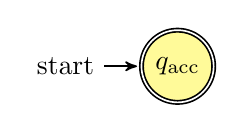
\begin{tikzpicture}[->,>=stealth',shorten >=1pt, auto, node distance=2cm, semithick]
  \tikzstyle{every state}=[text=black, fill=yellow!40]
  \node[initial,state,accepting] (q0)                    {$q_{\mathrm{acc}}$};
 ;
\end{tikzpicture}}
$\rangle$}  
& \text{if } x = \langle M, w \rangle \text{ for a Turing machine $M$ and string $w$}\\
& \qquad \qquad \text{ and } w \in L(M) \\

\scalebox{.5}{$\langle$ \hspace{-.5cm} \raisebox{-.4cm}{
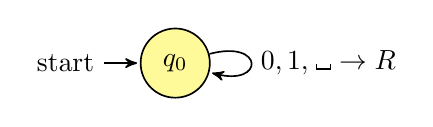
\begin{tikzpicture}[->,>=stealth',shorten >=1pt, auto, node distance=2cm, semithick]
  \tikzstyle{every state}=[text=black, fill=yellow!40]
  \node[initial,state] (q0)                    {$q_0$};
  \path (q0) edge  [loop right] node {$0, 1, \blank \to R$} (q0)
 ;
\end{tikzpicture}}
$\rangle$} 
& \text{otherwise}
\end{cases} 
\]


\item\gradeCorrect $\{w w \mid w \in \{0,1\}^* \} \le_m \{ w \mid w \in \{0,1\}^* \}$ and
\[
f(x) = \begin{cases}
w & \text{if } x = w w \text{ for a string $w$ over $\{0,1\}$}\\
\varepsilon & \text{otherwise}
\end{cases}
\]
\item\gradeCorrect $EQ_{\mathrm{TM}} \le_m A_{\mathrm{TM}}$ with 
\[
f(x) = \begin{cases}
 \scalebox{.7}{$\langle$ \hspace{-.5cm} \raisebox{-.4cm}{
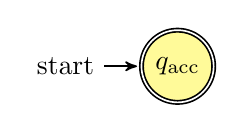
\begin{tikzpicture}[->,>=stealth',shorten >=1pt, auto, node distance=2cm, semithick]
  \tikzstyle{every state}=[text=black, fill=yellow!40]
  \node[initial,state,accepting] (q0)                    {$q_{\mathrm{acc}}$};
 ;
\end{tikzpicture}}
, $M_w \rangle$}  & \text{if } x = \langle M, w \rangle \text{ for a Turing machine $M$ and string $w$}\\\\
\varepsilon & \text{otherwise}.
\end{cases}
\]
Where for each Turing machine $M$, we  define 
\begin{align*}
    M_w = ``&\text{On input y} \\
    &1. \text{   Simulate $M$ on $w$.}\\
    &2. \text{   If it accepts, accept.}\\
    &3. \text{   If it rejects, reject."}
\end{align*}
You may assume that $\varepsilon$ is never a valid encoding and that encodings of pairs of Turing machines are never the same as encodings of a Turing machine and an input string (i.e., $\langle M_1, M_2 \rangle \neq \langle M_3, w \rangle$).

\end{enumerate}

%%%%%%%%%%% PROBLEM 3 %%%%%%%%%%%
\item \textbf{Computational histories} (10 points): \\
At any point in the computation of a Turing machine, we can 
record what is going on by (metaphorically) taking a ``snapshot''. 
We want this snapshot to contain all the information needed to simulate the rest of the computation. In particular, the snapshot encodes the
\begin{itemize}
\item Tape contents:  Although the tape is infinite, at any 
specific point in a computation, only finitely many cells have 
been used. These are the only relevant tape contents to be encoded.
\item Head position: An index to which position on the tape the head is currently pointing.
\item State: An index to which state in the finite control the computation is currently at.
\end{itemize}
Notice that much like the encoding  $\langle M \rangle$ of a 
Turing machine $M$, we can encode all of this snapshot 
information in a single string called a \emph{configuration} 
(usually denoted by the letter $C$). In the same spirit
of getter functions for components of encodings, all 
of the relevant information can effectively be extracted from 
the configuration. More formally, there is a computable 
function which computes each of the tape contents, head 
position, and state given a configuration as input. See Sipser 
Figure~3.4 (and surrounding discussion) for an explicit 
example of a configuration.

A computational history for Turing machine $M$ on input $w$ is 
sequence of configurations $C_1, C_2, \ldots, C_k$ such that 
configuration $C_{i+1}$ results from taking one step in the 
Turing machine computation corresponding to $C_i$
(in other words, one application of the transition
function). Additionally, $C_1$ is the starting configuration, 
corresponding to the tape that has the characters $w$ on 
the leftmost $|w|$-many cells of the tape, the tape head at 
the leftmost position, and the current state being the 
starting state of the Turing machine. We say that a 
computational history is {\it accepting} if the final 
configuration in the sequence $C_k$ has 
the current state being the accept state of the Turing machine.

Let's suppose we can describe both the encodings of Turing 
machines and configurations using the alphabet 
$\Sigma = \{0,1\}$. 
That is, $\langle M \rangle \in \Sigma^*$ and $C \in 
\Sigma^*$ for any Turing machine $M$ and configuration of the 
Turing machine $C$. We  define the language of accepting 
computational histories over the alphabet $\Gamma = \{0,1, 
2\}$:
\begin{align*}
H:= \{ \langle M \rangle 2 \langle w \rangle 2 C_1 2 \cdots 2 C_k \mid& ~M \textrm{ is a Turing machine, $w$ is a string,} \\
&C_1, \ldots, C_k \text{ is the computational history of } M \text{ on } w \\
&\text{and is accepting} \}
\end{align*}
That is, strings in the language $H$ start with an encoding of 
some Turing machine $M$, followed by an encoding of 
some string $w$, followed by an accepting computational 
history of $M$ on input $w$. There is a $2$ symbol between 
each of these components to serve as a delimiter. To be clear, 
each of these encodings is over the alphabet $\{0,1\}$, but 
you may also assume that it's possible to decide whether or 
not a particular bit string is an encoding of a Turing 
machine, a configuration, or neither.

\begin{enumerate}
\item\gradeCorrect Give a high-level description for 
a Turing machine that decides $H$ and justify 
why it works. Namely, prove that the Turing machine 
you define halts for each input and that it accepts
an arbitrary string if and only if that string is in $H$.
\item\gradeCompleteFirst Prove that $\SUBSTRING(H)$ is undecidable by showing a mapping reduction from $A_{\mathrm{TM}}$. That is, you will 
prove that $A_{\mathrm{TM}} \le_m \SUBSTRING(H)$
by giving a witnessing function. Recall that for any language $K \subseteq \Gamma^*$, we define 
\[
    \SUBSTRING(K) := \{ w \in \Gamma^* \mid \text{there exist } a,b \in \Gamma^* \text{ such that } awb \in K\}.
\]
Combining parts (a) and (b), notice that this implies that the 
class of decidable languages is not closed under the 
$\SUBSTRING$ operation. 

\end{enumerate}

%%%%%%%%%%% END PROBLEMS  %%%%%%%%%%%
\end{enumerate}

\end{document}